\usepackage[utf8]{inputenc}
\usepackage{amsmath, amssymb}
\usepackage{mathtools}
\usepackage{xcolor}
\usepackage{graphicx}
\usepackage[margin=1in]{geometry}
\usepackage{gensymb}
\usepackage{enumitem}
\documentclass{beamer}

\newcommand{\grad}{\vec{\nabla}}
\newcommand{\vvec}[1]{\begin{pmatrix}#1\end{pmatrix}}
\newcommand{\equation}[1]{\begin{equation}#1\end{equation}}
\newcommand{\mat}[1]{\begin{bmatrix}#1\end{bmatrix}}

% http://deic.uab.es/~iblanes/beamer_gallery/index_by_theme.html
% You can uncomment the themes below if you would like to use a different
% one:
%\usetheme{AnnArbor}
%\usetheme{Antibes}
%\usetheme{Bergen}
%\usetheme{Berkeley}
%\usetheme{Berlin}
%\usetheme{Boadilla}
%\usetheme{boxes}
%\usetheme{CambridgeUS}
%\usetheme{Copenhagen}
%\usetheme{Darmstadt}
%\usetheme{default}
%\usetheme{Frankfurt}
%\usetheme{Goettingen}
%\usetheme{Hannover}
%\usetheme{Ilmenau}
%\usetheme{JuanLesPins}
%\usetheme{Luebeck}
%\usetheme{Madrid}
\usetheme{Malmoe}
%\usetheme{Marburg}
%\usetheme{Montpellier}
%\usetheme{PaloAlto}
%\usetheme{Pittsburgh}
%\usetheme{Rochester}
%\usetheme{Singapore}
%\usetheme{Szeged}
%\usetheme{Warsaw}

%\setbeamertemplate{footline}[frame number]
\addtobeamertemplate{navigation symbols}{}{%
    \usebeamerfont{footline}%
    \usebeamercolor[fg]{footline}%
    \hspace{1em}%
    \insertframenumber/\inserttotalframenumber
}

\title{Speeding up Initial Data Generation in Einstein Toolkit}

\author{Vedant Puri\inst{1}\\ \and Roland Haas\inst{1} \and Eloisa Bentivegna\inst{2} }

\institute[University of Illinois,]
{
  \inst{1}University of Illinois
  \and
  \inst{2}%
  University of Catania, Italy
}
\date{11 May 2018}

\begin{document}

\begin{frame}\small
  \titlepage
\begin{flushright}
    
\includegraphics[scale=0.1]{einstein_right.jpg}
\end{flushright}
\end{frame}

\begin{frame}
\frametitle{Outline}
  \tableofcontents
\end{frame}

\section{Motivation}
\begin{frame}{Motivation}
  \begin{itemize}
    \item Modelling scenarios in astrophysics with numerical relativity simulations requires the production of suitable initial data sets.
    \item Initial data generated is needed for simulating black hole and neutron star mergers, cosmology and gravitational wave simulations.
    \item However, producing initial data is computationally intensive.
    \end{itemize}
% Any formulation involving GR has constraint equations (true at every point of time.)
\end{frame}

\begin{frame}{Initial Data}
    \begin{itemize}
        \item Obtained by solving constraint equations of general relativity together with equilibrium equations for matter.
        \item Laplacian dominated elliptic boundary value problems.
    \end{itemize}
\begin{center}
    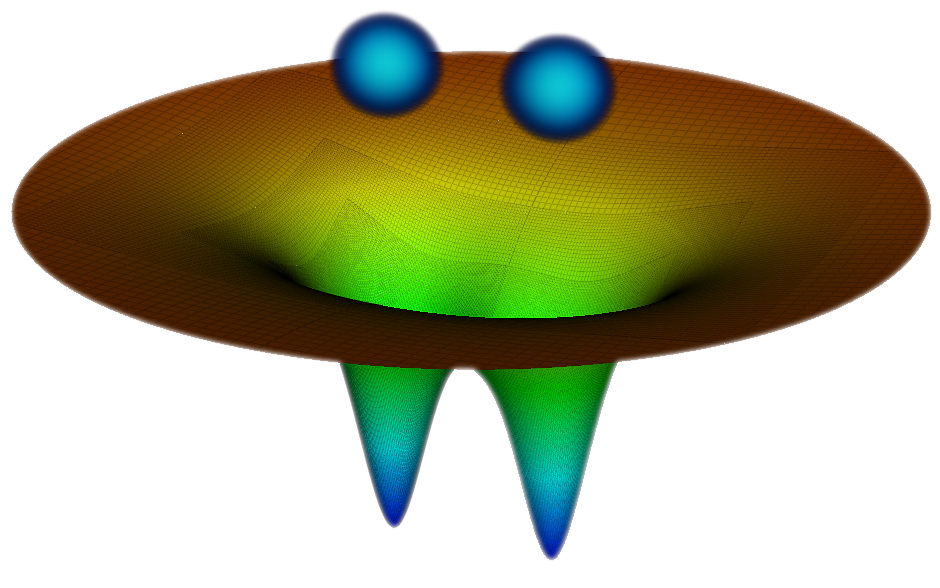
\includegraphics[scale=0.2]{bnsgrid.png} \\Metric for binary neutron star pair.
\end{center}
\end{frame}

\section{Einstein Toolkit}
\begin{frame}
\frametitle{Outline}
  \tableofcontents[currentsection]
\end{frame}

\begin{frame}{Einstein Toolkit}\small
Free open source, community toolkit for astrophysics simulations.
\begin{itemize}
    \item Cosmology
    \item Accretion disks after neutron star collisions
    \item Core collapse supernovae
    \item General relativistic magnetohydrodynamic simulations 
    \item Binary black hole, neutron star mergers
\end{itemize}

\begin{center}
    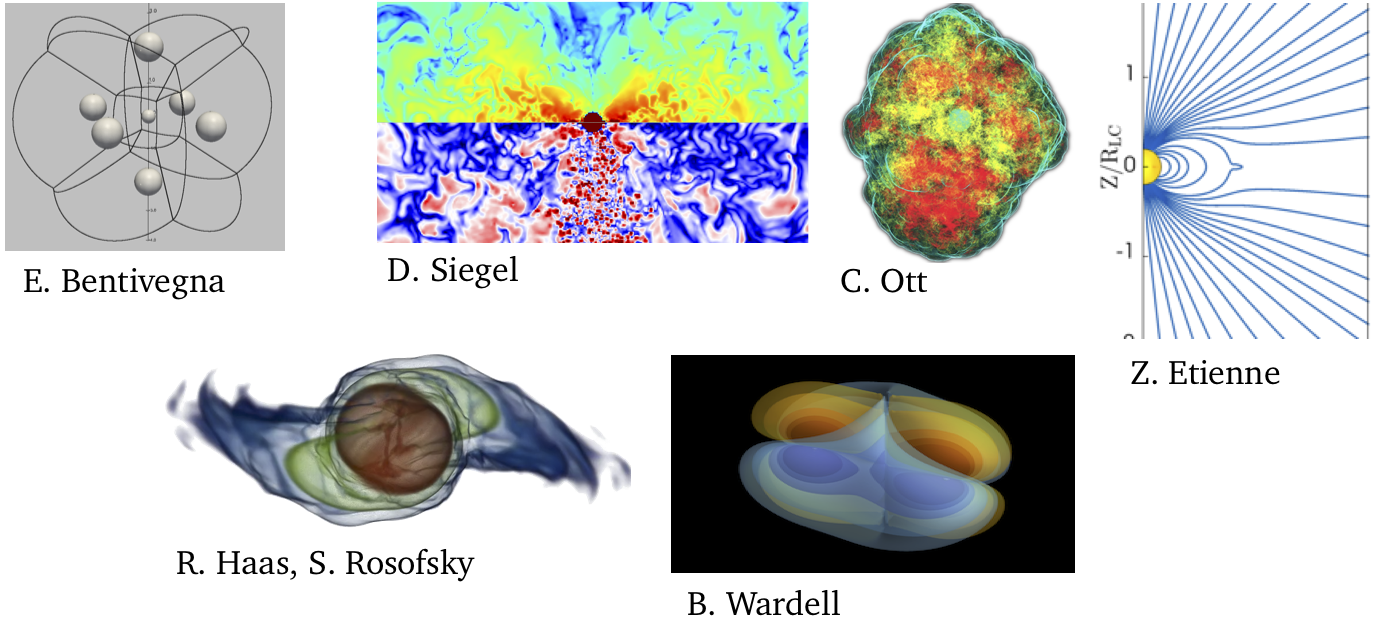
\includegraphics[scale=0.3]{ET1.png}
\end{center}
\begin{flushright}
    
\includegraphics[scale=0.1]{einstein_right.jpg}
\end{flushright}
\end{frame}

%%%%%%%%%%%%%%%%%%%%%%%%%%%%%%%%%%%%%%%%%%%%%%%%%%%%%%%%%%%%%%%%%%%%%%%%%%%%%%%%%%

\begin{frame}{CT\_Multilevel, a Multigrid Solver}\small
\begin{itemize}
    \item Existing multigrid solver in Einstein Toolkit developed by Eloisa Bentivegna. It is implemented using Cactus Computational Toolkit.
    \item Intended for cosmology and initial data problems.
    \item Multigrid solvers speed up convergence by passing the solution between a hierarchy of grids spanning the same space.
    
\end{itemize}
\begin{center}
    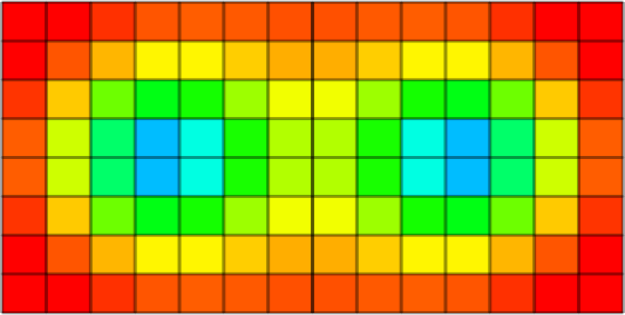
\includegraphics[scale=0.17]{grid0003.png}
    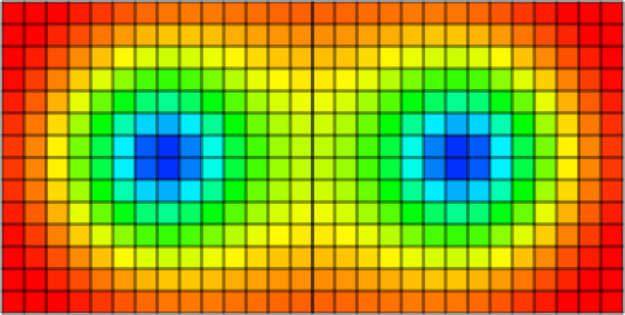
\includegraphics[scale=0.17]{grid0004.png} \\
    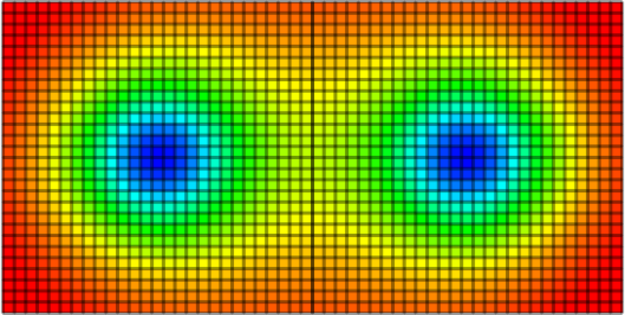
\includegraphics[scale=0.17]{grid0005.png}
\end{center}

% notes: Coarser grids pick up large scale features, and finer grids pick up local features to speed up convergence. CT_Multilevel currents works on Successive Overrelaxation Method with Gauss-Siedel. Smoothing means solving for the solution.   \item We intend to modify this smoothing operation with a faster method.
\end{frame}

\begin{frame}{Successive Over-Relaxation (SOR)}

\begin{itemize}
    \item At every grid, CT\_Multilevel solves a Dirichlet boundary value problem using SOR. It solves algebraic equation $Au=f$ iteratively:
    $$u_{i+1}=u_i+\omega(Au_i-f)$$
    \item SOR is extremely robust. It can handle nonlinear equations without any modifications.
    \item But it is slow.
    \item We intend to modify the smoothing operation, i.e. replace SOR with  a faster algorithm, while leaving the multigrid scheme intact.
\end{itemize}
\end{frame}

%%%%%%%%%%%%%%%%%%%%%%%%%%%%%%%%%%%%%%%%%%%%%%%%%%%%%%%%%%%%%%%%%%%%%%%%%%%%%%%%%%
\section{Scheduled Relaxation Jacobi}
\begin{frame}
\frametitle{Outline}
  \tableofcontents[currentsection]
\end{frame}

\begin{frame}{Scheduled Relaxation Jacobi (SRJ)}
\begin{itemize}
    \item SRJ (Adsuara et al, 2015) is an extension of Successive Over-Relaxation where a set of optimal $\omega$, relaxation factors, are precomputed to minimise the total number of iterations.
    $$u_{i+1} = u_i+\omega(Au-f)$$
    \item Since SRJ methodology has only been developed for linear equations, we linearize the equation using a Newton-Raphson scheme.
\end{itemize}

\end{frame}

\begin{frame}{Scheduled Relaxation Jacobi Results}
    \begin{center}
         $\triangle u+exp(x+y)u=(x^2+y^2+exp(x+y))e^{xy}$, 256x256 grid.
        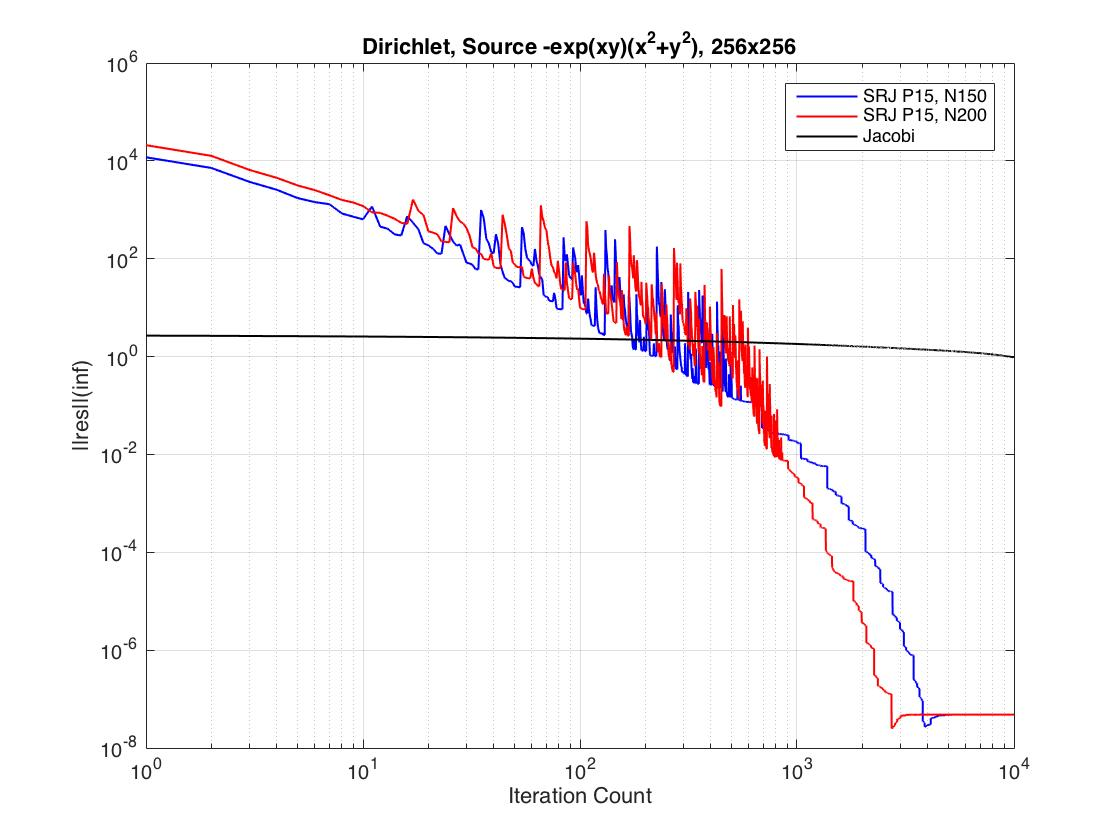
\includegraphics[scale=0.2]{exp(xy).jpg}
    \end{center}
\end{frame}

\begin{frame}{Scheduled Relaxation Jacobi Results}
    \begin{center}
        $\triangle u = u^3-\frac{3}{(x+1)^2(y+1)}-\frac{3}{(x+1)(y+1)^2}$, 256x256 grid.
        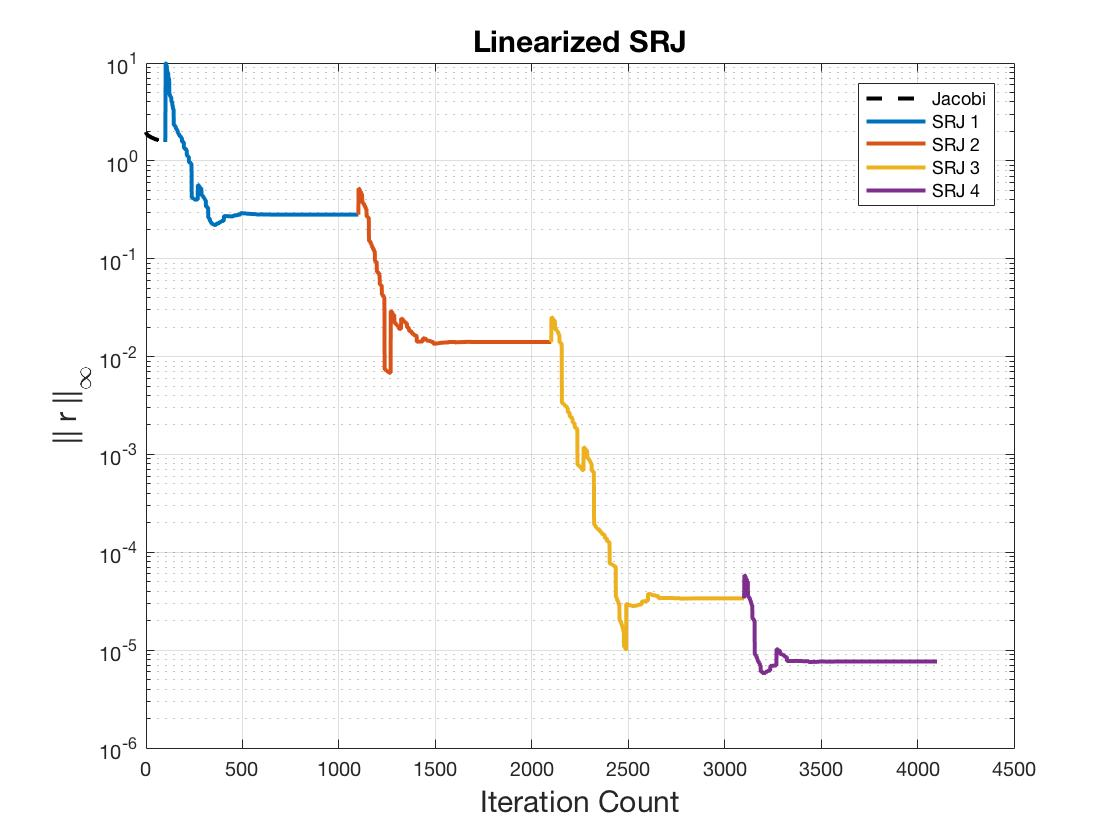
\includegraphics[scale=0.2]{SRJ.jpg}
    \end{center}
\end{frame}

\section{Preconditioned Krylov Subspace Method}
\begin{frame}
\frametitle{Outline}
  \tableofcontents[currentsection]
\end{frame}

\begin{frame}{Preconditioned Krylov Subspace Method (KSM)}
\begin{itemize}
    \item Krylov Subspace methods are a class of iterative linear solvers.
    \item A suitable preconditioner improves convergence rate.
    \item We linearize with Newton-Raphson scheme and solve using preconditioned KSM.
    \item We will only show results for linear equations because all methods share the same Newton-Raphson scheme.
\end{itemize}
\end{frame}

\begin{frame}{The Preconditioner}
A \textbf{preconditioner} is a lower order approximation to the inverse of a matrix. Since the Laplacian is the dominant term, we construct a preconditioner to solve for it directly. \\
\begin{itemize}
    \item Convert $\triangle u=f$ into an algebraic set of equations, $Mu=f$.
    \item Invert $M$ matrix-free using a discrete sine transform in $\mathcal{O}(N)$ complexity.
\end{itemize}
\end{frame}

\begin{frame}
 $\triangle u+exp(x+y)u=(x^2+y^2+exp(x+y))e^{xy}$, 500x500 grid.
 \begin{center}
     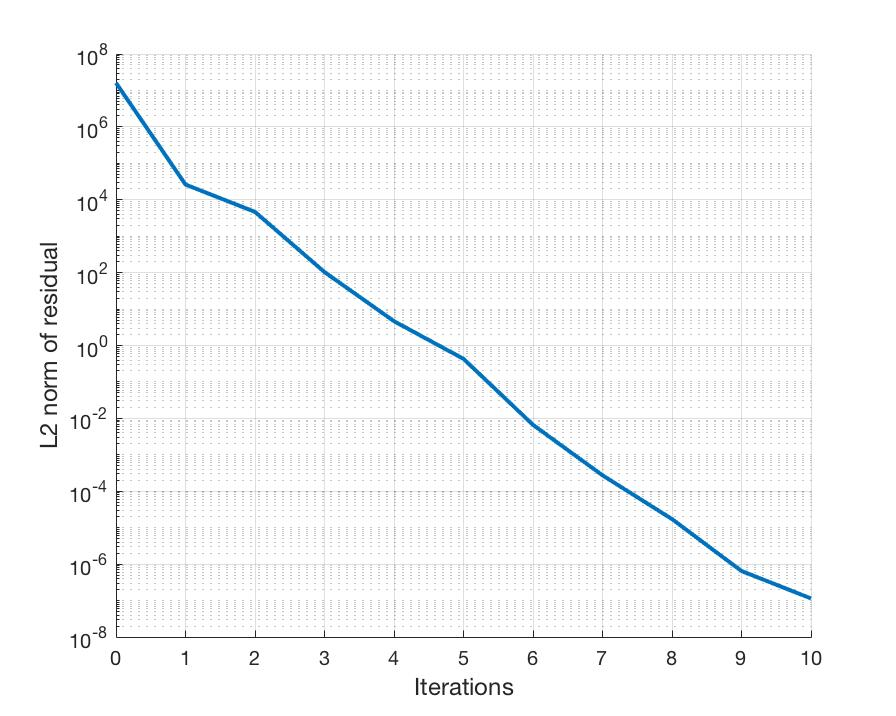
\includegraphics[scale=0.25]{res.jpg}
 \end{center}

\end{frame}

\begin{frame}
Solve$\triangle u+exp(x+y)u=(x^2+y^2+exp(x+y))e^{xy}$ for varying grid sizes.
\begin{center}
     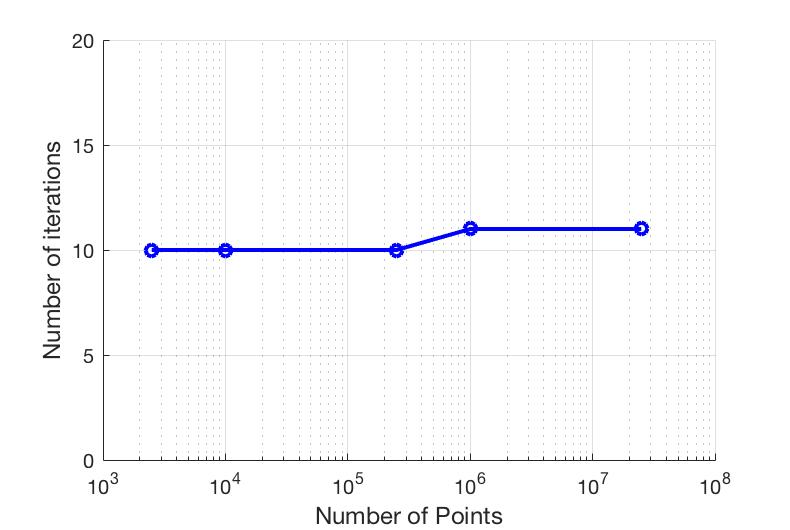
\includegraphics[scale=0.3]{iterations.jpg}
 \end{center}

\end{frame}

\section{Summary and Future Work}

\begin{frame}{Summary and Future Work}
\begin{itemize}
    \item We have two $\mathcal{O}(N)$ that reduce the number of iterations for a single grid.
    \item See how the schemes behaves inside a multigrid solver.
    \item Suitable treatment for the error equation?
    \item Implement in CT\_Multilevel.
\end{itemize}

\end{frame}

% \begin{frame}{}
% \begin{center}
%     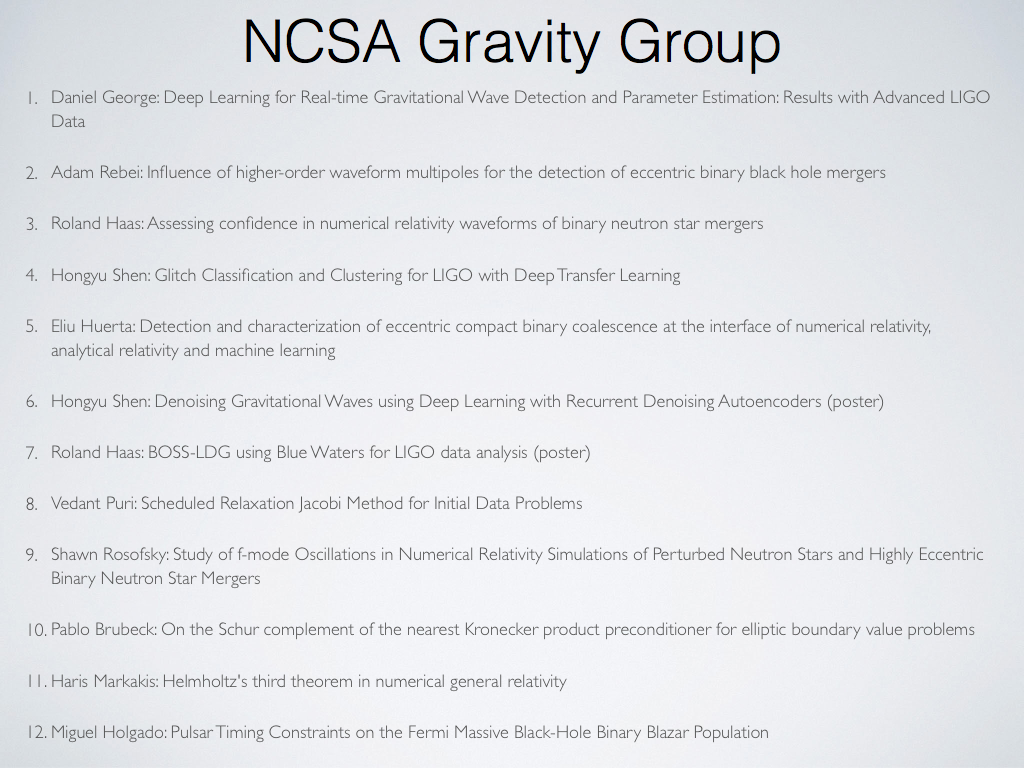
\includegraphics[scale=0.25]{GG.png}
% \end{center}
% \end{frame}

\begin{frame}{Einstein Toolkit}\small
Free open source, community toolkit for astrophysics simulations.
\begin{itemize}
    \item Cosmology
    \item Accretion disks after neutron star collisions
    \item Core collapse supernovae
    \item General relativistic magnetohydrodynamic simulations 
    \item Binary black hole, neutron star mergers
\end{itemize}

\begin{center}
    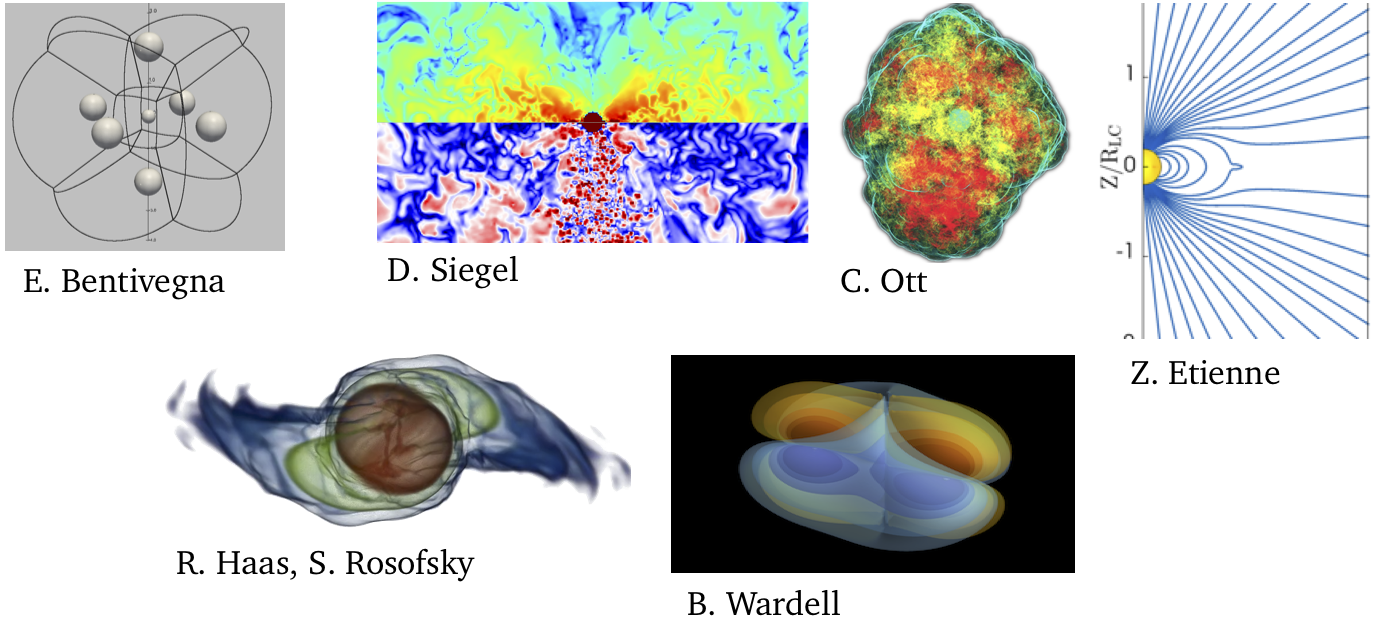
\includegraphics[scale=0.3]{ET1.png}
\end{center}
\begin{flushright}
    
\includegraphics[scale=0.1]{einstein_right.jpg}
\end{flushright}
\end{frame}


\end{document}
